\documentclass[12pt]{mitthesis}
\usepackage{lgrind, braket, amsmath, color, amssymb, bbm, booktabs}
\usepackage[pdftex]{graphicx}
\pagestyle{plain}

\newcommand{\TODO} [1]{\textcolor{magenta}{\textbf{TODO:} #1}}
\newcommand{\POINT}[1]{\textcolor{magenta}{\emph{#1}}}


\newcommand{\ts}{\tilde{s}\,}
\newcommand{\tl}{\tilde{\ell}\,}
\newcommand{\tm}{\tilde{m}\,}
\newcommand{\tsl}{\widetilde{s \ell}\,}

\begin{document}
\tableofcontents
\clearpage
\subsubsection*{NOTES}

\TODO{Remove old $\psi_{1,2}$ notation from figs.}

\TODO{Address width of SEELEM hole and relative widths of LIF/SEELEM
  distributions for distant doorway model.}

\TODO{Address relationship between relative fluorescence intensity and
  fractional bright state character.}

 \clearpage

 \chapter{Models of doorway-mediated intersystem crossing and their
   consequences in LIF and SEELEM spectra}
\label{chapter:models}

\section{Introduction}

The traditional basis set for intersystem crossing is diagonal in
``brightness.'' For the first excited state of closed-shell molecules,
it typically consists of a singlet bright state coupled directly to
many triplet dark states. This type of basis reflects the response of
the system to excitation by a photon, and is useful for understanding
systems in both the large molecule and small molecule limit. In the
small molecule limit, experimental results may often be deperturbed
explicitly due to the small number of interacting states. In the large
molecule limit, many states are involved in the interaction, and
analysis focuses on properties of the \emph{ensemble} of dark states
rather than the deperturbation of individual states.  As experimental
techniques evolve, the dividing line between small and large molecules
is pushed back, expanding the domain of complete deperturbation and
determinism.

In the intermediate case between the large and small molecule limits,
a few dark states may mediate the coupling between a bright state and
the remaining ensemble of dark states. When this happens, the directly
observable spectrum and the inferred dynamics of the system depend on
both the ensemble properties of the bath of dark states and the
individual properties of the mediating states (hereafter, doorway
states). Thus, an approach to intersystem crossing in the intermediate
case must combine the properties of the large and small molecule
limits.

A theory of the spectral signatures of doorway-mediated intersystem
crossing (DMISC) for systems containing a single bright state is
presented below. In section~\ref{sec:arrangements}, we discuss three
ways to re-formulate the problem of doorway-mediated coupling, derive
LIF intensity expressions for each, and compare the results.  In
section~\ref{sec:seelem-intensity}, we turn to evaluating terms in the
SEELEM intensity for doorway-mediated systems.  Using these intensity
expressions, we examine the spectral signatures of DMISC for several
model Hamiltonians.  The models examined are: a local doorway, a
distant doorway, a local doorway plus direct coupling, and a double
(local + distant) doorway.

%%%%%%%%%%%%%%%%%%%%%%%%%%%%%%%%%%%%%%%%%%%%%%%%%%%%%%%%%%%%%%%%%%%%%%
%%%%%%%%%%%%%%%%%%%%%%%%%%%%%%%%%%%%%%%%%%%%%%%%%%%%%%%%%%%%%%%%%%%%%%
%%%%%%%%%%%%%%%%%%%%%%%%%%%%%%%%%%%%%%%%%%%%%%%%%%%%%%%%%%%%%%%%%%%%%%

\section{Don't think of a doorway: three alternate arrangements of
  the effective Hamiltonian}
\label{sec:arrangements}

We begin with a simple doorway-mediated Hamiltonian arranged in the
traditional manner. A single bright basis state $\ket{s}$ is connected
to a single doorway basis state $\ket{\ell}$ by a spin-orbit matrix
element $H_{s \ell}$. The doorway basis state is, in turn, connected
to a block of prediagonalized dark states $\lbrace \ket{m} \rbrace$ by
a vector of matrix elements $\lbrace H_{\ell m} \rbrace$. Such a
Hamiltonian is shown in figure~\ref{fig:matrix-doorway}.

\begin{figure}
  \caption{Schematic of a doorway-mediated Hamiltonian. A single
    bright basis state $\ket{s}$ is connected to a single doorway
    basis state $\ket{\ell}$, which is, in turn, connected to a block
    of prediagonalized dark states $\lbrace \ket{m} \rbrace$.}
  \label{fig:matrix-doorway}
  \begin{equation*}
    \begin{bmatrix}
    E_s & H_{s \ell} \\
    & E_\ell & H_{\ell 1} & H_{\ell 2} & H_{\ell 3} & \dotsm \\
    & & E_1 \\
    & & & E_2 \\
    & & & & E_3 \\
    & & & & & \ddots \\
    \end{bmatrix}
  \end{equation*}
\end{figure}

This form of the Hamiltonian illustrates the dynamics of the system,
understood in terms of sequential intersystem crossing into a
heirarchy of coupled states. However, other patterns of interaction
between the bright state and the dark states are not immediately
apparent unless we do some more work.

A crucial quantity from the standpoint of dynamics is the fractional
bright state character of each eigenstate of the system. This
determines the radiative lifetime and absorption linestrength of
states observed in the spectrum. We examine this property for each
arrangement, and draw parallels between the results.

\subsection{The mixed basis}
\label{sec:mixed-basis}

% NEW!!!!!
Our first strategy for determining the distribution of fractional
bright state character among the dark states is to prediagonalize the
interaction between the bright state and the doorway state.  This
creates a new basis of ``mixed'' bright and doorway basis states,
which we refer to as the mixed basis.  From the mixed basis, we use
perturbaion theory to evaluate intensity lending among the dark
states.  
% Does this even make sense? Am I ruining this section?
Due to this use of perturbation theory in the second step, we consider
the mixed basis using a working assumption of a system in the strong
coupling limit, defined below.

The strong coupling limit of DMISC is characterized by a strong
doorway$\sim$bright state interaction compared to the average
doorway$\sim$dark state interaction. As a first step, the problem is
recast from a basis that contains one bright state and one doorway
state to a basis where the bright$\sim$doorway interaction is
diagonal.  The mixed bright and mixed doorway basis states are defined
as
\begin{equation}
  \label{eq:mixed-basis-def}
  \begin{split}
    \ket{\ts} & = (1-\alpha^2)^{1/2} \ket{s} + \alpha \ket{\ell} \\
    \ket{\tl} & = - \alpha \ket{s} + (1-\alpha^2)^{1/2} \ket{\ell},
  \end{split}
\end{equation}
where $\alpha$ is the bright$\sim$doorway mixing amplitude. Using this
basis, the prediagonalized block of mixed basis states is connected to
the prediagonalized block of dark states by an off-diagonal block of
matrix elements $H_{\ts m}$ and $H_{\tl
  m}$. Figure~\ref{fig:matrix-mixed} shows a schematic of the
Hamiltonian using a mixed basis.

\begin{figure}
  \caption{Schematic of a doorway-mediated ISC Hamiltonian after
    transformation to a mixed basis. The mixed basis states
    $\ket{\ts}$ and $\ket{\tl}$ have mixed bright$\sim$doorway
    character, and both have matrix elements with the ensemble of dark
    states.}
  \label{fig:matrix-mixed}
  \begin{equation*}
    \begin{bmatrix}
      E_{\ts} & & H_{\ts 1} & H_{\ts 2} & H_{\ts 3} & \dotsm \\
      & E_{\tl} & H_{\tl 1} & H_{\tl 2} & H_{\tl 3} & \dotsm \\
      & & E_1 \\
      & & & E_2 \\
      & & & & E_3 \\
      & & & & & \ddots \\
    \end{bmatrix}
  \end{equation*}
\end{figure}

Two rows of matrix elements connect the mixed states to the dark
states, suggesting two separate direct-coupled systems. However,
\textbf{correlations between the two rows of matrix elements make the
  distribution of fractional bright state character for a
  doorway-mediated system different from that of two direct-coupled
  systems.}  The matrix elements $H_{\ts m}$ and $H_{\tl m}$ can be
written in terms of the zero-order matrix element $H_{\ell m}$ and the
$\ket{s}$, $\ket{\ell}$ mixing amplitude $\alpha$:
\begin{equation}
  \begin{split}
    H_{\ts m} &= + \alpha H_{\ell m}\\
    H_{\tl m} &= + (1-\alpha^2)^{1/2} H_{\ell m}.
  \end{split}
\end{equation}
More patterns in bright state coupling through $\ket{\ts}$ and
$\ket{\tl}$ are apparent in the distribution of fractional
bright state character among the eigenstates of the system.

The fractional bright state character of any nominal dark state that
appears in the spectrum may be evaluated in terms of the mixed basis
using perturbation theory. We approximate the overlap of a nominal
dark state eigenfunction $\ket{M}$ with the bright state $\ket{s}$ by
making a first order correction to the dark state basis function
$\ket{m}$.  Using the mixed basis defined above,
\begin{equation}
  \label{eq:mixed-basis-overlap}
  \braket{M|s} = \alpha (1 - \alpha^2)^{1/2} H_{\ell m}
  \biggl \lbrace
    \frac{1}{\Delta E_{m \ts}} - \frac{1}{\Delta E_{m \tl}}
  \biggr \rbrace,
\end{equation}
The fractional bright state character of $\ket{M}$ may be written as
\begin{equation}
  \label{eq:mixed-basis-int}
  \lvert \braket{M|s} \rvert^2 = 
  \alpha^2 (1-\alpha^2) H_{\ell m}^2 
   \biggl \lbrace 
   \frac{1}{\Delta E_{m \ts}^2} +\frac{1}{\Delta E_{m \tl}^2} 
   - \frac{2}{\Delta E_{m \ts} \Delta E_{m \tl}}
   \biggr \rbrace.
\end{equation}
The three terms in this equation correspond to intensity lending
through the mixed bright state $\ket{\ts}$, the mixed doorway state
$\ket{\tl}$, and a cross term.  If this cross term is neglected, the
fractional bright state character of dark states behaves as \emph{two
  separate direct-coupled systems of equal coupling strength}, each
with an effective matrix element $\alpha (1-\alpha^2)^{1/2} H_{\ell
  m}$. The square terms dominate the intensity equation when $\Delta
E_{m \tl}$ becomes very large compared to $\Delta E_{m \ts}$ or
\emph{vice versa}.

The cross term is important when the energy difference
between the mixed basis states $\Delta E_{\ts \tl}$ is comparable in
magnitude to the coupling width $2 \pi \lvert \alpha^2 (1-\alpha^2)
H_{\ell m}^2 \rvert \rho_m$.
%If this is not the case, the effects of the cross term must be
%considered. 
The functional form of the cross term has several interesting
properties.  First, its sign does not depend on the relative signs of
the bright$\sim$doorway and doorway$\sim$dark matrix elements, only on
the relative signs of the energy denominators, $\Delta E_{m \ts}$ and
$\Delta E_{m \tl}$. The cross term, with its ($-$) sign included, is
\emph{always positive at energies that lie between those of the
  primary and secondary mixed states}, and negative outside this
range.

% The cross term diverges at the energies $E_{\ts}$ and $E_{\tl}$ of the
% mixed basis states, 
The cross term has a local minimum at the energy midpoint of the mixed
basis states, $\bar{E}_{s \ell} = (E_{\ts} + E_{\tl})/2$. The
fractional intensity increase for dark states due to the cross term,
in other words its ratio with respect to the sum of the square terms,
takes an especially simple form on an energy scale with zero chosen at
$\bar{E}_{s \ell}$,
\begin{equation}
  \label{eq:mixed-basis-ratio}
  \biggl( - \frac{2}{\Delta E_{m \ts} \Delta E_{m \tl}} \biggr) / 
  \biggl( \frac{1}{\Delta E_{m \ts}^2} +\frac{1}{\Delta E_{m \tl}^2} \biggr)
  \; = \; \frac{\Delta E_{\ts \tl} - \bar{E}_m}{\Delta E_{\ts \tl} + \bar{E}_m},
\end{equation}
where $\bar{E}_m = E_m - \bar{E}_{s \ell}$.  This ratio in Equation
\ref{eq:mixed-basis-ratio} depends only on the energy difference
$\Delta E_{\ts\tl}$ between the mixed basis states $\ket{\ts}$ and
$\ket{\tl}$, and is independent of both the bright$\sim$doorway mixing
coefficient and the doorway$\sim$dark matrix element.  The cross term
ratio from equation~\ref{eq:mixed-basis-ratio} is plotted in
figure~\ref{fig:local-cross-term} along with the three terms in the
expression for fractional bright state character, equation
\ref{eq:mixed-basis-int}.

\begin{figure}
  \caption{Shown in the plot are contributions to the fractional
    bright state character in a nominal dark eigenstate $\ket{M}$
    arising from three terms: borrowing through the mixed basis state
    $\ket{\ts}$, borrowing through the other mixed basis state
    $\ket{\tl}$, and a cross term.  Also shown is the ratio of the
    cross term to the square terms, exhibiting a maximum at the energy
    midpoint between $E_{\ts}$ and $E_{\tl}$.}
  \label{fig:local-cross-term}
  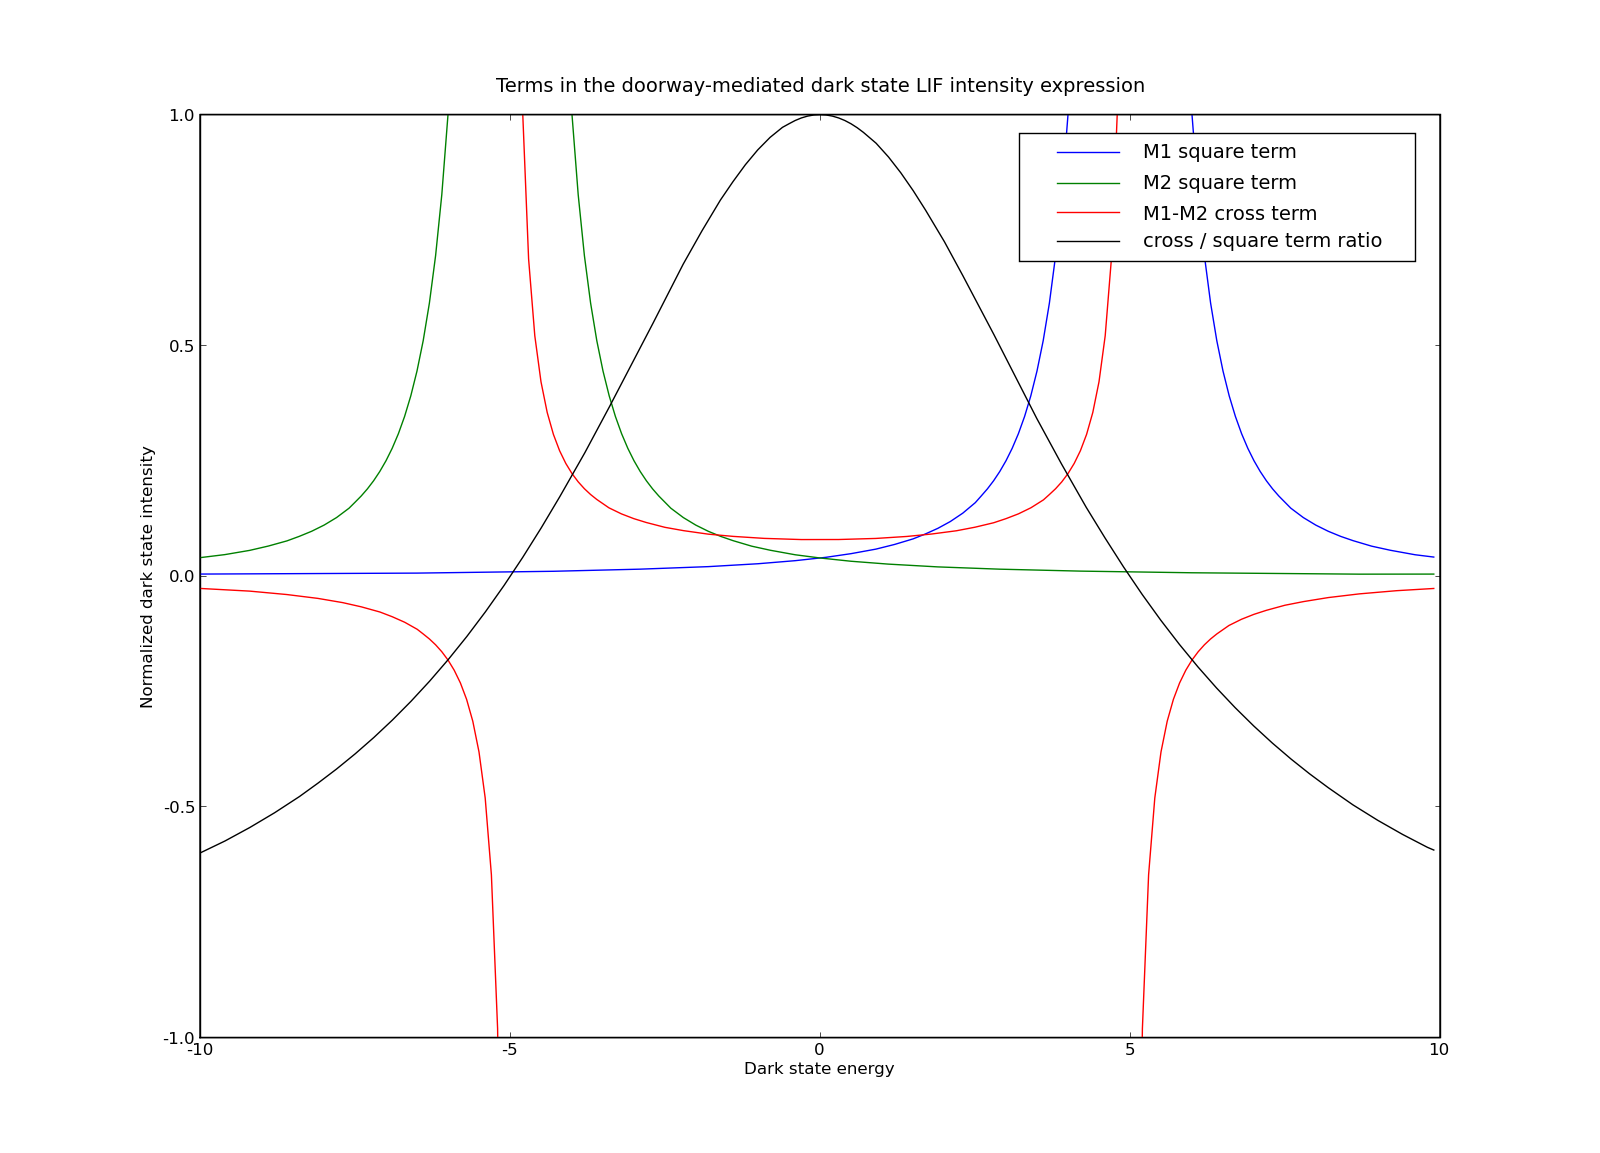
\includegraphics[width=8in, angle=90]{local-doorway-terms.png}
\end{figure}

The equation for fractional bright state character of a dark state in
the $\ket{s}$, $\ket{\ell}$ mixed basis contains two classes of terms:
square terms and a cross term. The square terms are equivalent in the
vicinity of each mixed state, and can be considered as appropriate for
two separate, equal-magnitude, direct-coupled systems of dark
states. These quasi-direct systems interact via the cross term, which
\emph{always} skews the intensities of the dark states toward the
energy midpoint of the mixed basis states. Moreover, the fractional
contribution of the cross term to the fractional bright state
character is independent of the matrix elements of the system.

\subsection{The embedded bright state arrangement}
\label{sec:ebsa}

In the limit of weak doorway$\sim$bright coupling compared to the average
doorway$\sim$dark coupling, we can take the opposite approach with respect
to perturbation theory. Here, the doorway$\sim$dark interactions are
diagonalized, and perturbation theory is used to evaluate the
remaining bright$\sim$doorway interaction. The results of this analysis
will be compared to the equations from the strong coupling regime, and
an instructive correspondence will be made.

The effective Hamiltonian is re-ordered so the bright state is
embedded among the dark states.  After re-ordering, the Hamiltonian is
equivalent in form to a direct-coupled system, with the doorway state
occupying the position normally held by the bright state.  A schematic
diagram of this arrangement is shown in figure~\ref{fig:matrix-ebsa}.

\begin{figure}
  \caption{Schematic of a doorway-mediated Hamiltonian arranged
    according to the embedded bright state picture. The form of the
    matrix is equivalent to a direct coupling model.}
  \label{fig:matrix-ebsa}
  \begin{equation*}
    \begin{bmatrix}
      E_\ell & H_{\ell 1} & H_{\ell 2} & H_{\ell s} & H_{\ell 3} & \dotsm \\
      & E_1 \\
      & & E_2 \\
      & & & E_s \\
      & & & & E_3 \\
      & & & & & \ddots \\
    \end{bmatrix}
  \end{equation*}
\end{figure}

To derive equations for the fractional bright state character of a
nominally dark eigenstate, we adopt separate strategies in the vicinity
of the bright state $\ket{s}$ and doorway state $\ket{\ell}$.  In the
vicinity of $\ket{s}$, contamination of dark states by the bright
state may be evaluated by making a second-order correction to the dark
state wavefunction.  This yields a fractional bright state character
of
\begin{equation}\label{eq:ebsa-bright-int}
\lvert \braket{M|s} \rvert^2 = 
    \frac{H_{s\ell}^2 H_{\ell m}^2}{\Delta E_{ms}^2 \Delta E_{m\ell}^2}.
\end{equation}

To compare this expression with the mixed basis results, one
adjustment must be made. Since we are evaluating dark state
intensities in the vicinity of $E_s$, $\lvert \Delta E_{ms} \rvert \ll
\lvert \Delta E_{s\ell} \rvert$, and $\lvert \Delta E_{m\ell} \rvert
\approx \lvert \Delta E_{s\ell} \rvert$. In light of this
approximation, the fractional bright state character becomes
\begin{equation}\label{eq:ebsa-bright-int-approx}
  \frac{H_{s\ell}^2 H_{\ell m}^2}{\Delta E_{ms}^2 \Delta E_{s\ell}^2} \approx 
  \alpha^2 H_{\ell m}^2 \frac{1}{\Delta E_{ms}^2},
\end{equation}
since $\alpha \approx H_{s\ell} / \Delta E_{s\ell}$.
Using this, we look for an equivalence with the mixed basis intensity
formula, equation \ref{eq:mixed-basis-int}:
\begin{equation*}
  \alpha^2 (1-\alpha^2) H_{\ell m}^2 
   \biggl \lbrace 
   \frac{1}{\Delta E_{m \ts}^2} +\frac{1}{\Delta E_{m \tl}^2} 
   - \frac{2}{\Delta E_{m \ts} \Delta E_{m \tl}}
   \biggr \rbrace.
\end{equation*}
Since the bright$\sim$doorway coupling is weak, two approximations to
the mixed basis results are appropriate:
\begin{equation}
  \label{eq:weak-coupling-approx}
  \begin{split}
    (1 - \alpha^2)^{1/2} &\approx 1 \\
    (E_{\ts}, E_{\tl}) &\approx (E_s, E_{\ell}).
  \end{split}
\end{equation}
With these approximations, the mixed basis expression becomes:
\begin{equation}
  \label{eq:mixed-basis-int-approx}
  \alpha^2 H_{\ell m}^2 
   \biggl \lbrace 
   \frac{1}{\Delta E_{ms}^2} +\frac{1}{\Delta E_{m\ell}^2} 
   - \frac{2}{\Delta E_{ms} \Delta E_{m\ell}}
   \biggr \rbrace,
\end{equation}
and it is clear that our result for the embedded bright state
arrangement in the vicinity of $\ket{s}$ (equation
\ref{eq:ebsa-bright-int-approx}) is equal to the square term for
borrowing from the bright state in the mixed basis.

We now turn to deriving an expression for fractional bright state
character in the vicinity of the doorway state $\ket{\ell}$.  Since
the doorway$\sim$dark interactions are strong, the effective Hamiltonian is
diagonalized in the vicinity of the doorway state, forming a set of
prediagonalized states $\lbrace \ket{\tm} \rbrace$.  Each state in
this doorway block $\ket{\tm}$ is a linear combination of dark and
doorway states:
\begin{equation}
  \label{eq:ebsa-block}
  \ket{\tm} = C_{\ell \tm} \ket{\ell} + \sum_m C_{m \tm} \ket{m}.
\end{equation}
After diagonalization of the doorway block, mixing between the
zero-order bright state and the doorway block states may be evaluated
using perturbation theory. The doorway component $\ket{\ell}$ of each
diagonalized state $\ket{\tm}$ is contaminated to first order with
bright state amplitude
\begin{equation}
  \label{eq:ebsa-inblock-overlap}
  \braket{\ell\,^{(1)}|s} = - \frac{H_{s\ell}}{\Delta E_{s\ell}},
\end{equation}
and the dark state components $\ket{m}$ are not. From this equation,
the fractional bright state character in $\ket{\tm}$ follows
immediately,
\begin{equation}
  \label{eq:ebsa-inblock-int}
  \lvert \braket{\tm|s} \rvert^2 =
  C_{\ell \tm}^2 \frac{H_{s\ell}^2}{\Delta E_{s\ell}^2}.
\end{equation}

To compare the above expression with the mixed basis formulas,
we rewrite equation \ref{eq:ebsa-inblock-int} using the
perturbation-theoretic approximation for $C_{\ell\tm}$, $H_{\ell\tm} /
\Delta E_{\ell\tm}$:
\begin{equation}
  \label{eq:ebsa-inblock-int-approx}
  C_{\ell \tm}^2 \frac{H_{s\ell}^2}{\Delta E_{s\ell}^2} \approx
  \frac{H_{\ell \tm}^2}{\Delta E_{\ell \tm}^2} 
  \frac{ H_{s\ell}^2}{ \Delta E_{s\ell}^2} \approx
  \alpha^2 H_{\ell \tm}^2 \frac{1}{\Delta E_{\ell \tm}^2}.
\end{equation}
Adjusting for notation, this is equal to the second term of the mixed
basis equation.  Thus, the embedded bright state result for the doorway
block plays the role of the square term for the mixed doorway basis
state in the earlier formulation.

The effective Hamiltonian for doorway mediated intersystem crossing in
the weak bright-doorway coupling limit has been rearranged to account
for relatively strong doorway$\sim$dark interactions. This is called the
embedded bright state arrangement, because the bright state has
``switched places'' with one of the dark states in the traditional
direct-coupling Hamiltonian. After using a combination of
diagonalization and perturbation theory to analyze the intensity
distribution of dark states, the results from this arrangement were
shown to correspond to the square terms in the strong coupling
limit. Thus, the intensity expressions from the embedded bright state
arrangement emerge as a subset of the mixed basis equations.

The consequences of the embedded bright state arrangement extend
beyond the evaluation of systems in the weak coupling limit.  The fact
that the Hamiltonian can be arranged to have the same form as a
direct-coupling Hamiltonian has ramifications for eigenstate energies
and spectral deconvolution; we discus these at length in a later
chapter.

\subsection{Formulation as a complex-energy effective
  Hamiltonian}
\label{sec:complex-energy}

As a third alternative, the dynamics of intensity lending to a bath of
dark states can be viewed as a process of irreversible decay from the
bright and doorway basis states into a quasi-continuum of dark
states. The decay widths are embedded into the energies of the bright
and doorway basis states by adding an imaginary component, $E =
\epsilon -i \Gamma / 2$. Because the effects of dark state coupling
are folded into the bright and doorway states, the complex energy
formulation reduces the doorway-canonical Hamiltonian to a 2-level
system.

The complex-energy Hamiltonian for a single doorway system may be
written as
\begin{equation}
  \label{eq:complex-h}
  \mathbf{H} = 
  \begin{bmatrix}
    \epsilon_s & V_{s\ell} \\
    V_{s\ell} & \epsilon_{\ell} - i \Gamma_{\ell} / 2 \\
  \end{bmatrix}.
\end{equation}
The width of the doorway state is related to the average doorway$\sim$dark
matrix element by the golden rule relation $\Gamma_{\ell} = 2 \pi \langle
V_{\ell m}^2 \rangle \rho_{m}$.

Results for a two-level complex-energy Hamiltonian are derived in
detail in chapter 9 of reference [REF: Bob's book]. Following the
derivation therein, we rewrite the Hamiltonian as two terms:
\begin{equation}
  \label{eq:complex-zero}
  \mathbf{H} = 
  (\bar{\epsilon}_{s\ell} - i \bar{\Gamma}_{s\ell} / 2) 
  \mathbf{I} +
  \begin{bmatrix}
    \delta \epsilon_{s\ell} - i \delta \Gamma_{s\ell} / 2 & V_{s\ell} \\
    V_{s\ell} & - (\delta \epsilon_{s\ell} - i \delta \Gamma_{s\ell} / 2) \\
  \end{bmatrix}.
\end{equation}
The re-centered energies have the values
\begin{subequations}
  \label{eq:energy-defs}
  \begin{align}
    \bar{\epsilon}_{s\ell} & = (\epsilon_s + \epsilon_{\ell}) / 2 \\
    \delta \epsilon_{s\ell} & = (\epsilon_s - \epsilon_{\ell}) / 2.
  \end{align}
\end{subequations}
Since the bright state is not connected to the bath of dark states in
a doorway-mediated Hamiltonian, $\Gamma_s = 0$, and
\begin{subequations}
  \label{eq:gamma-defs}
  \begin{align}
    \bar{\Gamma}_{s\ell} & = \Gamma_{\ell} / 2 \\
    \delta \Gamma_{s\ell} & = - \Gamma_{\ell} / 2.
  \end{align}
\end{subequations}

\begin{figure}
  \caption{Widths of the nominal bright and doorway eigenstates in a
    complex-energy doorway Hamiltonian. To demonstrate the weak
    coupling regime (left), the coupling matrix element $V_{s\ell}$ is
    set to 0.25 times the magnitude of the doorway width
    $\Gamma_{\ell}$. For the intermediate coupling regime (center),
    $V_{s\ell}=\Gamma_{\ell}$; for the strong coupling regime (right),
    $V_{s\ell}=4\Gamma_{\ell}$.}
  \label{fig:complex-widths}
  \centering
  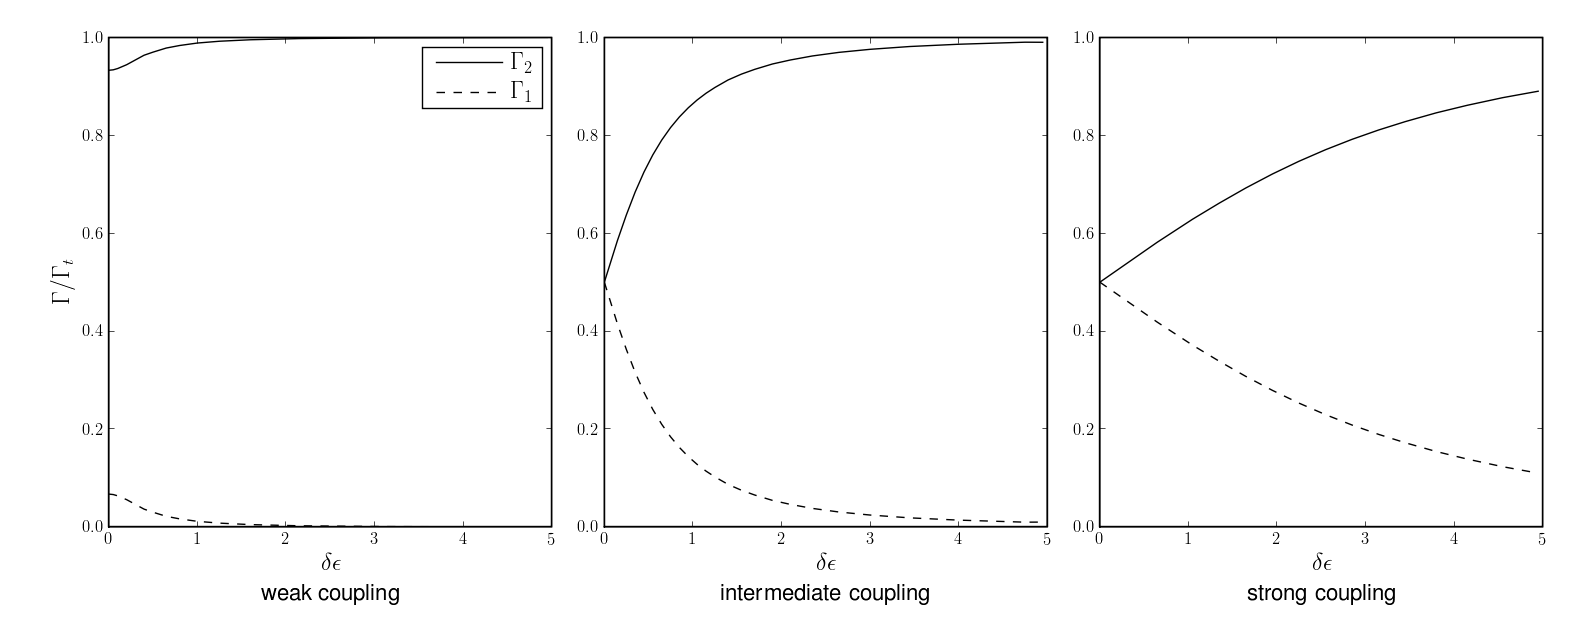
\includegraphics[angle=90, height=7.4in]{complex-widths.png}
\end{figure}

Diagonalization of this Hamiltonian leads to level repulsion in the
real components of the energy, as for real Hamiltonians.  However, the
imaginary components of the eigenvalues are closer to the average
width $\Gamma_{\ell}/2$, as the bright state borrows some decay width
from the doorway state.

Figure~\ref{fig:complex-widths} shows the width of the nominal singlet
and triplet eigenstates of equation~\ref{eq:complex-h} for several
magnitudes of bright$\sim$doorway coupling.  In the weak coupling
regime, $V_{s\ell} \ll \Gamma_{\ell}$. The bright state borrows little
width from the doorway state, even when the difference in real energy,
$\delta \epsilon_{s\ell}$, is zero. In the intermediate coupling
regime, the eigenstate widths converge to the average width
$\Gamma_{\ell}/2$ when $\delta \epsilon_{s\ell} = 0$. In the strong
coupling case, the difference in the widths $\ket{S}$ and $\ket{L}$
approaches $\Gamma_{\ell} / 2$ less rapidly as $\delta
\epsilon_{s\ell}$ increases.

We now turn to evaluating the dark state intensity distribution using
the complex energy formulation.  The energies and widths of the
eigenstates $\ket{S}$ and $\ket{L}$ are given by the real and
imaginary parts of their eigenvalues:
\begin{subequations}
  \label{eq:complex-eigenvals}
  \begin{align}
    \epsilon_{S}& = 
      \bar{\epsilon}_{s \ell} \pm Re \left ( \mathcal{E} \right ) &
    \Gamma_{S}& = 
      \bar{\epsilon}_{s \ell} \pm Im \left ( \mathcal{E} \right ) \\
    \epsilon_{L}& = 
      \bar{\epsilon}_{s \ell} \mp Re \left ( \mathcal{E} \right ) &
    \Gamma_{L}& = 
      \bar{\epsilon}_{s \ell} \mp Im \left ( \mathcal{E} \right )
  \end{align}
\end{subequations}
where the energy eigenvalue $\mathcal{E}$ is given by
\begin{equation}
     \mathcal{E} = \sqrt{(\delta \epsilon_{s\ell} - i \delta \Gamma_{s\ell} / 2)^2 
       + V_{s\ell}^2},
\end{equation}
and the choice of sign in equation \ref{eq:complex-eigenvals} is given
by the sign of $\delta \epsilon_{s \ell}$ in equation
\ref{eq:energy-defs}.  We must also determine the bright state
character of the eigenstates $\ket{S}$, $\ket{L}$.  The bright state
amplitudes are obtained from the eigenvectors of the Hamiltonian,
\begin{subequations}
  \begin{align}
    \alpha_S =
    \braket{\tilde{S}|s}& = 
     \sqrt{\frac
       {(\delta \epsilon_{s\ell} - i \delta \Gamma_{s\ell}/2) + \mathcal{E}}
       {2 \mathcal{E}}} \\
     \alpha_L =
     \braket{\tilde{L}|s}& = 
     \sqrt{\frac
       {(\delta \epsilon_{s\ell} - i \delta \Gamma_{s\ell}/2) - \mathcal{E}}
       {2 \mathcal{E}}}.
   \end{align}
\end{subequations}
With these tools in hand, we evaluate the intensity distribution by
deriving the absorption cross section for the system in terms of the
Green's function $G(E) = \lim_{\gamma \rightarrow 0} \left [
  \mathbf{H} - (E+i \gamma) \mathbf{I} \right ]^{-1}$:
\begin{equation}
\sigma(E) \propto Im(\braket{g|\mu G(E) \mu|g}).
\end{equation}
When the Green's function is evaluated over the eigenvectors of
$\mathbf{H}$, only two diagonal elements remain:
\begin{equation}
  \label{eq:greens-func}
  \begin{split}
    Im \, G(E) =
    \lvert \alpha_{S} \rvert^2
    \frac{\Gamma_{S}}
         {(\epsilon_{S} - E)^2 + \Gamma_{S}^2}
    + \lvert \alpha_{L} \rvert^2
    \frac{\Gamma_{L}}
         {(\epsilon_{L} - E)^2 + \Gamma_{L}^2}. 
  \end{split}
\end{equation}
Therefore, the intensity distribution for the complex energy
Hamiltonian is the sum of two Lorentzian functions, with energies and
widths given by the eigenvalues of the Hamiltonian, and weigted in
magnitude by the fractional bright state character.

\begin{figure}
  \caption{Dark state intensity distributions for a doorway coupled
    system where $\delta \epsilon_{s\ell} = 0.5$ and $\delta
    \Gamma_{s\ell} = 1$. Three coupling regimes result from the
    relative magnitude of $V_{s\ell}$: weak coupling ($V_{s\ell} =
    \delta \Gamma_{s\ell} / 10$), intermediate coupling ($V_{s\ell} =
    \delta \Gamma_{s\ell}$), and strong coupling ($V_{s\ell} = 10
    \delta \Gamma_{s\ell}$). Note the different scales of both the x
    and y axes for each plot. The widths $\Gamma_S$ of the $\ket{S}$
    intensity term are $0.005 \, \Gamma_{\ell}$, $0.26 \,
    \Gamma_{\ell}$, and $0.48 \, \Gamma_{\ell}$ for the weak,
    intermediate, and strong coupling regimes, respectively.}
  \label{fig:complex-overlaps}
  \centering
  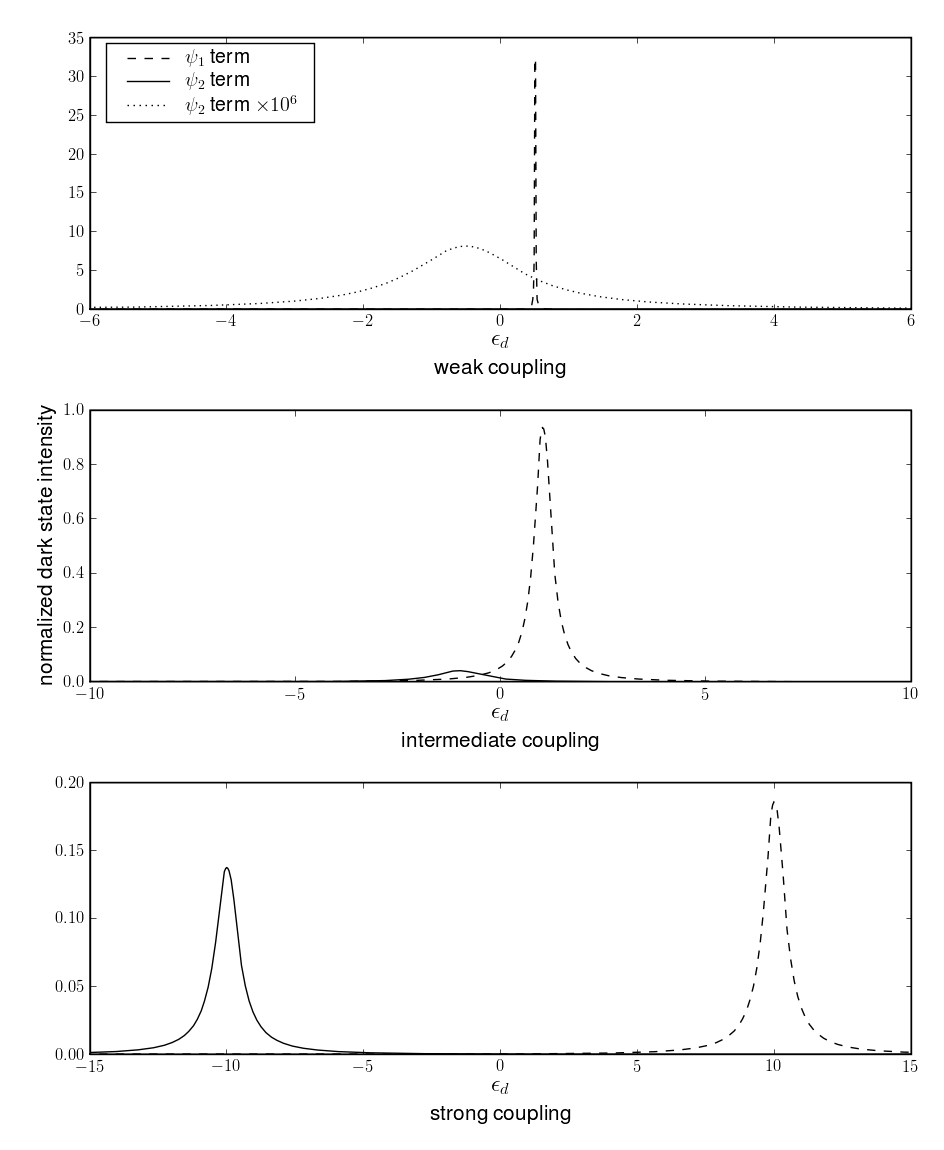
\includegraphics[width=6.4in]{complex-overlaps.png}
\end{figure}

\begin{table}
  \caption{Eigenstate energy difference and width of the nominal
    bright eigenstate $\ket{S}$ for the systems depicted in 
    Figure~\ref{fig:complex-overlaps}.  In the weak coupling regime, 
    the energy separation of the eigenstates $\ket{S}$ and $\ket{L}$ 
    is approximately that of the zero-order states $\ket{s}$ and 
    $\ket{\ell}$.  The nominal bright eigenstate $\ket{S}$ borrows 
    little coupling width from the dorway state, and remains narrow.
    In the strong coupling regime, the eigenstates are
    separated in energy by $2V_{s\ell}$ and have similar widths.}
  \label{table:complex-int-params}
  \centering
  \begin{tabular}{rlrr}
    & \\
    \toprule
    $V_{s\ell} / \delta \Gamma_{s\ell}$ & Coupling regime & $\delta
    \epsilon_{SL} / \delta \epsilon_{s\ell}$ & $\Gamma_S / \Gamma_{\ell}$ \\
    \midrule
    $1/10$ & Weak & $1.02$ & $0.005$ \\
    $1$ & Intermediate & $2.06$ & $0.257$ \\
    $10$ & Strong & $20.00$ & $0.475$ \\
    \bottomrule
  \end{tabular}
\end{table}
Figure~\ref{fig:complex-overlaps} shows the terms of equation
\ref{eq:greens-func} for each of the three coupling regimes. In order
to show details of the intensity distribution for each regime, the
scale of the axes was adjusted for each subplot. Although the scales
were chosen carefully to show the general trends in the distributions,
the plots cannot simultaneously and clearly communicate the
dramatic changes in $\delta \epsilon_{SL}$ and $\Gamma_S$ as the
magnitude of $V_{s\ell}$ changes. For this reason, these quantities
are listed in table~\ref{table:complex-int-params}.

\begin{figure}
  \caption{A comparison of the intensity distribution results from
    direct diagonalization (solid line) and perturbation theory
    (dashed line) in the weak coupling regime.}
  \label{fig:complex-compare-weak}
  \centering
  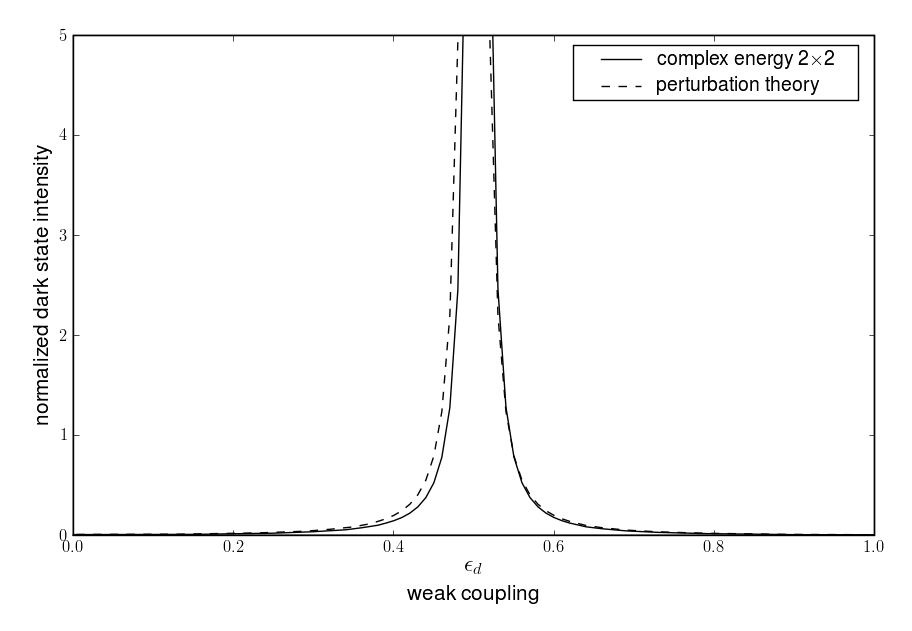
\includegraphics[width=6in]{complex-compare-weak.png}
\end{figure}

In the weak coupling regime, the nominal bright eigenstate $\ket{S}$
is much narrower than that of the nominal doorway eigenstate
$\ket{L}$, which remains nearly at its original width.  To compare
with our earlier results from the embedded bright state picture, we
analyze the weakly coupled system presented above in terms of the
perturbation theory developed in the previous section.
Figure~\ref{fig:complex-compare-weak} shows a comparison between the
complex Hamiltonian results and those derived from perturbation theory
using equation~\ref{eq:ebsa-bright-int}. To make this comparison, the
effective matrix element $V_{\ell d}$ was calculated from the width
$\Gamma_\ell$ of the doorway state using the golden rule. The
perturbation results show only a slight offset in energy, due to the
use of the approximation $\epsilon_{S} \approx \epsilon_{s}$.

\begin{figure}
  \caption{A doorway-mediated Hamiltonian in the strong coupling
    limit, where the mixing is complete in both the real and imaginary
    parts of the eigenfunctions.}
  \label{fig:complex-compare-strong}
  \centering
  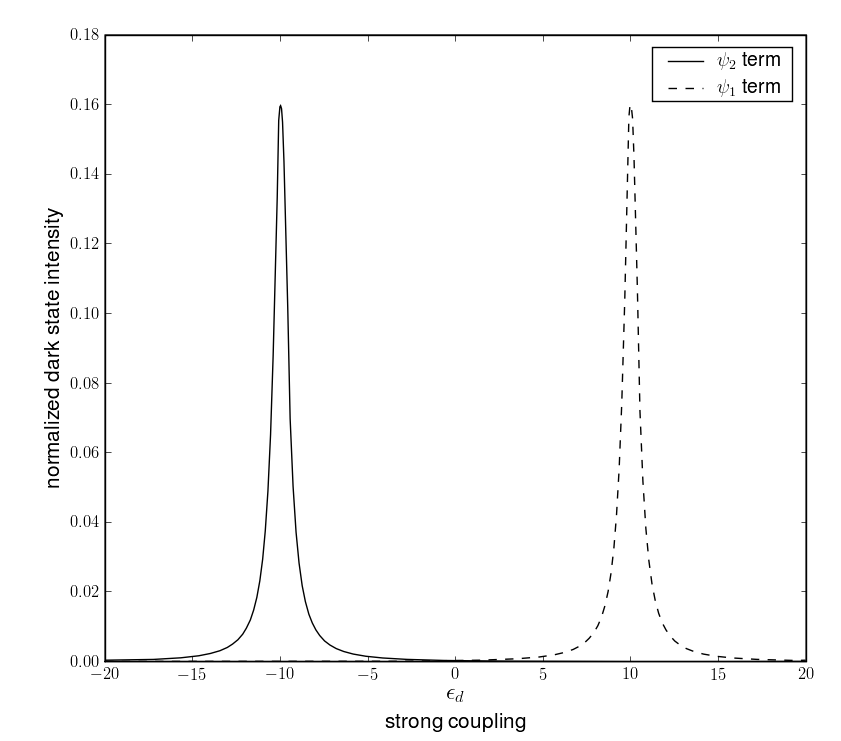
\includegraphics[width=6in]{complex-compare-strong.png}
\end{figure}

In the strong coupling regime, we make a qualitative comparison to the
earlier results derived for the mixed basis.  The strong coupling
intensity formula, equation~\ref{eq:mixed-basis-int}, predicts
identical dark state intensity distributions in the vicinity of both
the bright and doorway states.  In the bottom plot of
figure~\ref{fig:complex-overlaps}, it can be seen that the system is
approaching this limit.  A more extreme example is shown in
figure~\ref{fig:complex-compare-strong}, where the zero-order (real)
energy spacing $\delta \epsilon_{s\ell}$ has been decreased to $0.01 \,
\delta \Gamma_{s\ell}$. In this case, the mixing between $\ket{S}$ and
$\ket{L}$ is complete in both intensity (real part) and width
(imaginary part).

A complex energy effective Hamiltonian has been used to reduce the
doorway-mediated coupling problem to a two level system. The dark
state intensity distribution was presented graphically for the weak,
intermediate, and strong coupling regimes. The distributions derived
from diagonalizing the $2 \times 2$ complex energy Hamiltonian were
shown to have the same trends as those obtained using perturbation
theory for the mixed basis and the embedded bright state picture.
Like the results from the embedded bright state arrangement, the
complex energy Hamiltonian formula does not include a cross term in
the distribution of fractional bright state character.  We will return
to the complex energy formulation later in the chapter when we
consider the local doorway plus direct coupling model.

%%%%%%%%%%%%%%%%%%%%%%%%%%%%%%%%%%%%%%%%%%%%%%%%%%%%%%%%%%%%%%%%%%%%%%
%%%%%%%%%%%%%%%%%%%%%%%%%%%%%%%%%%%%%%%%%%%%%%%%%%%%%%%%%%%%%%%%%%%%%%
%%%%%%%%%%%%%%%%%%%%%%%%%%%%%%%%%%%%%%%%%%%%%%%%%%%%%%%%%%%%%%%%%%%%%%

\section{Doorway-mediated coupling and SEELEM intensity distribution}
\label{sec:seelem-intensity}

In a molecular beam experiment, detection by surface electron ejection
by laser-excited metastables (SEELEM) produces a spectrum that is
sensitive to eigenstates with only a small amount of fractional bright
state character.  This detection channel is complementary to
laser-induced fluorescence, which is sensitive to eigenstates
containing a large amount of fractional bright state character.  The
intensity information in a SEELEM spectrum, in conjunction with LIF,
provides a complete description of the distribution of fractional
bright state character among an ensemble of predominantly dark
eigenstates. However, the relationship between SEELEM intensity and
fractional bright state character is somewhat more complicated than it
is for LIF.  In this section, we derive SEELEM intensity expressions
and discuss interference between detection pathways involving the
bright and doorway basis state.

An eigenstate $\ket{M}$ of a doorway-coupled system is written as a
linear combination of the zero-order bright state, doorway state, and
dark states:
\begin{equation}
  \ket{M} = C_s \ket{s} + C_{\ell} \ket{\ell} + \sum_m C_m \ket{m}
\end{equation}
The SEELEM detection probability for a molecule in eigenstate
$\ket{M}$ is modeled as the product of three factors: excitation
probability, survival probability, and electron ejection
probability. The excitation probability is proportional to the
fractional bright state character:
\begin{equation}
  P_{ex} = A_{ex} C_s^2
\end{equation}
where $A_{ex}$ is a constant factor for the bright state in question.

Following Altunata, we write the survival probability
in terms of the bright state character \cite{altunata00}:
\begin{equation}
  P_{surv} = exp \left( -R_m C_s^2 \right).
\end{equation}
The factor $R_m$ is defined as ratio of flight time in the molecular
beam to the fluorescence lifetime of a pure bright state:
\begin{equation}
  R_m = \frac{t_{\text{flight}}}{\tau_s}.
\end{equation}
The molecular beam flight time $t_{\text{flight}}$ is a constant for
the experiment, while the pure bright state lifetime $\tau_s$ is a
property of the bright state in question.

The electron ejection probability is more complicated, since it
depends on the probability of de-excitation to the ground state upon
impact with the metal surface.  If the energy released upon
de-excitation is greater than the work function of the metal, an
electron may be ejected from the metal surface and detected with an
electron multiplier.

Normally, the metal surface used for SEELEM detection is chosen such
that the vertical excitation energy of the bright state is greater
than the work function of the metal. However, the doorway state may
also contain enough vertical excitation energy to eject electrons from
the metal surface. In this case, there is an additional possibility
that interference between the phases of bright and doorway amplitudes
in $\ket{M}$ might lead to changes in the total angle-energy averaged
electron cross section. We address these complications by separating
the electron ejection probability into three terms: a bright state
term, a possible doorway term, and a possible cross term:
\begin{equation}
  \begin{split}
    P_{ej} =& \; P_{ej}^{(s)} + P_{ej}^{(\ell)} + P_{ej}^{(\times)}\\ 
    =& A_{ej}^{(s)} C_s^2 + A_{ej}^{(\ell)} C_\ell^2 + A_{ej}^{(\times)} C_s C_\ell
  \end{split}
\end{equation}
We examine each term separately, creating for example a SEELEM
detection probability term $P_{SEELEM}^{(s)}$ that includes only the
bright state term $P_{ej}^{(s)}$ from the electron ejection
probability factor.  The results for each can be summed to determine
the total detection probability.

\subsection{The bright state term}
\label{sec:bright-state-term}

We begin with the bright state term for the SEELEM detection probability:
\begin{equation}
  \label{eq:seelem-prob-s}
  \begin{split}
    P_{SEELEM}^{(s)} &= P_{ex} \times P_{surv} \times P_{ej}^{(s)}\\
    &= \left( A_{ex} \, A_{ej}^{(s)} \right) C_s^4 \; exp \left( -R_m
      C_s^2 \right).
  \end{split}
\end{equation}
As a function of $C_s^2$, $P_{SEELEM}^{(s)}$ has the form of a
chi-square distribution with six degrees of freedom, a fact
better illustrated by making the substitution $x \equiv 2 C_s^2 /
R_m$:
\begin{equation}
  \label{eq:seelem-prob-chisq}
  P_{SEELEM}^{(s)} \propto x^{6/2 - 1} \; exp \left( - \frac{x}{2} \right).
\end{equation}
%An example of this distribution is shown in figure ????.

%\TODO{Figure: SEELEM intensity distribution, bright state term.}

To gain insight into the energy dependence of the SEELEM detection
probability for an ensemble of dark states with average doorway state
coupling $\langle H_{\ell m}^2 \rangle$, we evaluate the form of the
SEELEM detection probability for a single eigenstate $\ket{M}$ as a
function of energy.  To carry this out, we note that the only
energy-dependent parameter in the above equation is the fractional
bright state character, $C_s^2$.

The maximum of the SEELEM intensity distribution is found by taking
the derivative of the SEELEM detection probability with respect to
energy:
\begin{equation}
    \frac{\partial P_{SEELEM}^{(s)}}{\partial E} = 
       A^{(s)} \, P_{surv} \, C_s^2 \; \frac{\partial C_s^2}{\partial E} 
       \left( 2 - R_m C_s^2 \right)
\end{equation}
Setting this expression to zero, we obtain a maximum for
$P_{SEELEM}^{(s)}$ where
\begin{equation}
  C_s^2 = \frac{2}{R_m}.
\end{equation}
Substituting this quantity into the SEELEM detection probability
(equation~\ref{eq:seelem-prob-s}), we arrive at a maximum intensity of
\begin{equation}\label{eq:seelem-max-s}
  A^{(s)} \left( \frac{2}{e R_m} \right)^2.
\end{equation}
This is a surprising result: the maximum SEELEM detection probability
is independent of the matrix elements of the Hamiltonian! 

The width of the intensity distribution does not share this
invariance.  To find the half width, we first make the approximation
that the survival probability is approximately unity on the outer edge
of the intensity distribution. Setting the total probability to half
the quantity from equation~\ref{eq:seelem-max-s} and rearranging to
find $C_s^2$, we get
\begin{equation}
  \label{eq:seelem-half-s}
  C_s^2 = \frac{\sqrt{2}}{e R_m} 
\end{equation}
at the half maximum.

Up to this point, we have used no perturbation theory in our
derivation. The results above depend only on the adopted functional
form of the SEELEM detection probability.  To arrive at a final
expression for the width, we use perturbation theory to determine the
quantity $C_s^2$ as a function of energy in the weak and strong
coupling limits.

In the weak coupling limit, equation \ref{eq:ebsa-bright-int-approx}
from the bright state arrangement relates $C_s^2$ to the energy
denominator $\Delta E_{\ell m}$:
\begin{equation}
  C_s^2 = \alpha^2 \frac{H_{\ell m}^2}{\Delta E_{ms}^2}.
\end{equation}
Solving for $\Delta E_{ms}$, the FWHM of the distribution
is determined to be
\begin{equation}
  \label{eq:seelem-weak-fwhm}
  \text{FWHM} = 2 \lvert \alpha H_{\ell m} \mathcal{C}_{\frac{1}{2}}\rvert,
\end{equation}
where $\mathcal{C}_{\frac{1}{2}}^2$ is the fractional bright state
character at the SEELEM half-maximum, determined in
equation~\ref{eq:seelem-half-s}.  The energy dependence of the
intensity expression in the weak coupling limit arises only from a
squared energy denominator $\Delta E_{ms}$, thus the distribution is
an even function when the energy zero is chosen to be the bright state
energy $E_s$.

In the strong coupling limit, the energy dependence of $C_s^2$ is more
complicated. Equation~\ref{eq:mixed-basis-int} gives the relation:
\begin{equation}
  C_s^2 = \alpha^2 (1-\alpha^2)H_{\ell m}^2
  \left \lbrace
    \frac{1}{\Delta E_{m \ts}} -
    \frac{1}{\Delta E_{m \tl}}
  \right \rbrace^2
\end{equation}
in the mixed basis.  As explained in section~\ref{sec:mixed-basis},
the distribution of bright state intensity in the strong coupling
limit is symmetric about the energy midpoint $\bar{E}_{\ts \tl}$ of
the mixed basis states.  We can remove one of the energy denominators
by rewriting the equation using the energy difference $\Delta E_{\ts
  \tl}$.  Making the substitutuion $\Delta E_{m \tl} = \Delta E_{m
  \ts} + \Delta E_{\ts \tl}$,
\begin{equation}
  C_s^2 = \alpha^2 (1-\alpha^2)H_{\ell m}^2
  \left \lbrace
    \frac{\Delta E_{\ts \tl}}
    {\Delta E_{m \ts}(\Delta E_{m \ts} + \Delta E_{\ts \tl})}
  \right \rbrace^2.
\end{equation}
The FWHM of the distribution around either $E_{\ts}$ or $E_{\tl}$ is
given by the solutions to a quadratic equation:
\begin{equation}
  \text{FWHM} = \left \lbrace
    4 \left \lvert
      \alpha (1-\alpha^2)^{1/2}H_{\ell m} \Delta E_{\ts \tl} 
      \mathcal{C}_{\frac{1}{2}}
      \right \rvert + \Delta E_{\ts \tl}^2
  \right \rbrace^{\frac{1}{2}}.
\end{equation}

We have derived the widths of the bright state term of the SEELEM
intensity distribution in both the weak and strong coupling limits.
Along the way, a maximum of the distribution was found that depends
only on the quantity $R_m$, which is a constant of the experiment and
the molecule being studied.  A value of fractional bright state
character was determined for the half-maximum of the distribution,
which also depends only on $R_m$.  Since our use of perturbation
theory was limited to the final steps of the derivation, most of the
properties determined above depend only on the functional form of
$P_{SEELEM}^{(s)}$.  We turn next to the doorway term for SEELEM
detection probability, and compare its properties to those of the bright state
term.

\subsection{The doorway term}

If the doorway state has sufficient vertical excitation energy,
%  Franck-Condon overlap with
% low-lying vibrational levels of the ground state, 
it may contribute
to the electron ejection probability. We turn now to derive an
intensity distribution for the doorway term
\begin{equation}
  P_{SEELEM}^{(\ell)} = \left( A_{ex} A_{ej}^{(\ell)} \right) 
    C_s^2 C_\ell^2 \; exp \left( -R_m C_s^2 \right).
\end{equation}

Because the amplitudes of the bright and doorway states are squared in
this equation, the relative phase of the bright vs. doorway
contributions cannot lead to interference in this term. Going further, the
fact that the system is doorway-mediated suggests that the doorway
character be parametrized as a function of the bright state
character:
\begin{equation}
  C_{\ell}^2 = f(C_s^2).
\end{equation}
We derive this relationship separately for the weak and strong
coupling regimes.

In the weak coupling regime, we can invert the results from the
embedded bright state arrangement
(equation~\ref{eq:ebsa-bright-int-approx}) to determine an expression
for $f_{weak}$:
\begin{equation}
  f_{weak} \left ( C_s^2 \right ) = C_s^2 \frac{\Delta E_{s\ell}^2}{H_{s\ell}^2}
\end{equation}
This gives a SEELEM detection probability proportional to the bright
state term,
\begin{equation}
  \begin{split}
    P_{SEELEM, weak}^{(\ell)} &= 
    \left( A_{ex} A_{ej}^{(\ell)} \right) 
    C_s^2 \left ( C_s^2 \frac{\Delta E_{s\ell}^2}{H_{s\ell}^2} \right )
    \; exp \left( -R_m C_s^2 \right)\\
    &= \frac{\Delta E_{s\ell}^2}{H_{s\ell}^2} \; P_{SEELEM}^{(s)},
  \end{split}
\end{equation}
the properties of which are discussed in the preceding section.

In the strong coupling regime, we begin by using the mixed basis to
derive the fractional doorway state character in a nominally dark
eigenstate $\ket{M}$:
\begin{equation}
  \lvert \braket{M|\ell} \rvert^2 = 
  H_{\ell m}^2 \left \lbrace
    \frac{\alpha^2}{\Delta E_{m \ts}} +
    \frac{(1-\alpha^2)}{\Delta E_{m \tl}}
  \right \rbrace^2.
\end{equation}
The function $f_{strong}$ does not collapse into a simple form as it
does for the weak coupling regime.  We write the function instead in
terms of $\lvert \braket{M|s} \rvert^2$ and $\lvert \braket{M|\ell}
\rvert^2$,
\begin{equation}
  \begin{split}
    f_{strong} &= \frac{C_s^2}{C_{\ell}^2}\\
    &= \frac{\lvert \braket{M|s} \rvert^2}
    {\lvert \braket{M|\ell} \rvert^2},\\
  \end{split}
\end{equation}
referring the reader to the expression for $\lvert \braket{M|s}
\rvert^2$ in equation~\ref{eq:mixed-basis-int}.  We note that the
doorway$\sim$dark matrix element $H_{\ell m}$ cancels out in the
function $f_{strong}$, since it appears to the same power in $\lvert
\braket{M|s} \rvert^2$ and $\lvert \braket{M|\ell} \rvert^2$.  Unlike
the weak coupling regime, $f_{strong}$ is a function of the energy
differences $\Delta E_{m \ts}$ and $\Delta E_{m \tl}$.  Cross terms
involving these energy denominators always appear with a $(-)$ sign in
the numerator and a $(+)$ sign in the denominator, so they have the
effect of decreasing the SEELEM detection probability.  The
bright$\sim$doorway mixing amplitude $\alpha$ appears only to even
powers in $f_{strong}$, so interference effects do not arise from the
phase of this mixing amplitude.  

% Figure ???? shows the bright state
% and doorway state SEELEM intensity terms in the strong coupling limit,
% for comparison.

% \TODO{Figure: bright state and doorway state SEELEM intensity terms in
%   the strong coupling limit.}

We have derived the form of the doorway term for SEELEM detection
probability for the weak and strong coupling limits.  In the weak
coupling limit, the doorway term is simply proportional to the bright
state term.  In the strong coupling limit, the form of the doorway
term is more complicated, but does not include any interference effects
arising from coupling to the bright state through the doorway state.

\subsection{The cross term}

If the doorway state has sufficient Franck-Condon overlap with
low-lying vibrational levels of the ground state \emph{and} the
angle-energy integrated \emph{total} cross section for electron
ejection is affected by interference between the bright and doorway
pathways, the electron ejection cross term may contribute to the
intensity distribution. The form of the cross term
\begin{equation}
  P_{SEELEM}^{(\times)} = \left( A_{ex} A_{ej}^{(\times)} \right)
    C_s^3 C_\ell exp \left( -R_m C_s^2 \right)
\end{equation}
contains odd powers of $C_s$ and $C_{\ell}$, and according to their
relative phase, may add or subtract from the square terms.
Interference effects arising from the cross term in the SEELEM
detection probability are discussed in detail by Selen Altunata
\cite{altunata00, altunata02, altunata-thesis}.  Since we observe no
such effects in the experiments described in this thesis, we do not
give the cross term further consideration.

% If the doorway$\sim$dark matrix elements are assumed to have random
% phase, the relative phase of $C_s$ and $C_{\ell}$ is determined only
% by the energy of the dark state relative to the zero order primary
% and secondary mixed basis states. TODO: PROVE THIS FOR STRONG AND
% WEAK COUPLING
% % TODO!!!!!!!
% The highly lopsided SEELEM intensity distributions observed in the
% $V^3_0K^1_0$ vibrational subband of $S_1$ acetylene were originally
% attributed to effects of the electron ejection cross term; however, in
% a later chapter we show that the inferred matrix element between the
% bright state and the local doorway state is not sufficient to produce
% such effects without the presence of a stronger, distant doorway.

%%%%%%%%%%%%%%%%%%%%%%%%%%%%%%%%%%%%%%%%%%%%%%%%%%%%%%%%%%%%%%%%%%%%%%
%%%%%%%%%%%%%%%%%%%%%%%%%%%%%%%%%%%%%%%%%%%%%%%%%%%%%%%%%%%%%%%%%%%%%%
%%%%%%%%%%%%%%%%%%%%%%%%%%%%%%%%%%%%%%%%%%%%%%%%%%%%%%%%%%%%%%%%%%%%%%

\section{The local doorway model}
\label{sec:model-local}

We turn now to examine several model Hamiltonians for doorway-mediated
systems, using the tools developed earlier in the chapter.  These
models are really classifications of the types of spectra that may
appear for molecules exhibiting doorway-mediated coupling.  Each model
combines an appropriate basis set for evaluating the LIF and SEELEM
intensity distributions with an assumption as to the range of states
observed in the spectrum.

The basis set for a local doorway model was introduced in
section~\ref{sec:arrangements}, and has been used throughout the
chapter. It includes a single bright basis state $\ket{s}$, a single
doorway basis state $\ket{\ell}$, and a set of $N$ pre-diagonalized
dark basis states $\lbrace \ket{m} \rbrace$.  The single bright basis
state $\ket{s}$ carries all oscillator strength for the system, and
thus plays a crucial role in the detectability of all states.  All
matrix elements between $\ket{s}$ and the bath of dark states are
zero.

Upon diagonalization, the effective Hamiltonian yields a set of $N$
nominally dark eigenstates $\lbrace \ket{M} \rbrace$, as well as two
``special'' eigenstates $\ket{S}$ and $\ket{L}$.  The state $\ket{S}$
contains the greatest fractional bright state character, and likewise
the state $\ket{L}$ contains the single greatest fractional doorway
basis character.  A cursory look at the LIF spectrum will reveal
$\ket{S}$ immediately, because it carries the greatest amount of
oscillator strength.

The final defining criterion for a local doorway model is that the
eigenstate $\ket{L}$ is observed in the spectrum.  This model does not
carry in its definition any assumptions about the relative magnitudes
or distributions of the remaining nonzero matrix elements in the
effective Hamiltonian; it can include systems in the strong or weak
coupling limits.

We have already examined the distribution of LIF intensity in
section~\ref{sec:arrangements}.  Likewise, we used the local doorway
model as a template for deriving the width of the SEELEM intensity
distribution in section~\ref{sec:seelem-intensity}.  As we move on to
other models, we focus on differences from the results for the local
doorway model.

% Wishes:
%
% Width and skewness of the LIF intensity distribution
% Width and variance of the SEELEM distribution
% Discussion of the ``SEELEM hole'' and how it relates to the variance
% of the LIF distribution.
% SEELEM skewness about the nominal bright state -- introduce
% interference here.

\section{The distant doorway model}
\label{sec:model-distant}

The distant doorway model differs from the local doorway model in that
the nominal doorway state is not observed in the spectrum.  In the
limit that the doorway-bright energy difference becomes large compared
to the width of dark state coupling in the vicinity of the bright
state, statistical intensity metrics cannot distinguish a distant
doorway from a system characterized by direct coupling.  However,
evidence for doorway-mediated coupling can still be obtained through
other means, and under these circumstances the distant doorway model
will provide some indication of the relative coupling magnitudes and
the energy of the nominal doorway state.

Since $\ket{\ell}$ is well separated from the bright state in energy,
some approximations to the dark state intensity distributions can be
made.  For a distant doorway, the bright state energy denominator
dominates the intensity formula (equation \ref{eq:mixed-basis-int}),
and
\begin{equation}
  \label{eq:distant-lif}
  \begin{split}
  \lvert \braket{M|s} \rvert^2& = 
  \alpha^2 (1-\alpha^2) H_{\ell m}^2 
   \biggl \lbrace 
   \frac{1}{\Delta E_{m \ts}} +\frac{1}{\Delta E_{m \tl}}
   \biggr \rbrace^2\\
   & \approx \alpha^2 \frac{H_{\ell m}^2}{\Delta E_{m \ts}^2}.\\
   \end{split}
\end{equation}
In addition to eliminating one energy denominator from the above
equation, we have also made the approximation that $(1-\alpha^2)
\approx 1$.  This approximation is fairly good (5\% error) if
$\ket{s}$ and $\ket{\ell}$ are mixed to less than 25\%.  The SEELEM
intensity distribution above is equivalent to the weak coupling
formula in section\ref{sec:bright-state-term}.

If a spectrum is observed in the vicinity of the bright state and a
distant doorway model is assumed, the question can be asked: what is
the energy of $\ket{L}$, the nominal doorway state?  The properties of
the LIF and SEELEM intensity distributions in the vicinity of the
bright state do not yield the energy of $\ket{L}$ directly.  However,
the product $\lvert \alpha \langle H_{\ell m} \rangle_{rms} \rvert$
can be estimated from the width of the SEELEM spectrum, using
equation~\ref{eq:seelem-weak-fwhm}.  From this quantity, we
parametrize $\alpha$ in terms of $\Delta E_{s\ell}$ and predict the
LIF/SEELEM intensity of $\ket{L}$ as a function of energy separation
from the bright state.

An expression for $\alpha$ in terms of $\Delta E_{s\ell}$ and the matrix
element $H_{s\ell}$ comes from the analytical solution to the $2 \times
2$ Hamiltonian in the mixed basis:
\begin{equation}
  \begin{split}
    \alpha^2& = 
      \frac{\left ( 2 H_{s\ell} \right )^2}{
          \left (
            \Delta E_{s\ell} + 
            \sqrt{\Delta E_{s\ell}^2 + 4 H_{s\ell}^2}
          \right )^2
          + 4 H_{s\ell}^2
      }\\
      & \approx \frac{H_{s\ell}^2}{\Delta E_{s\ell}^2}.\\
      \end{split}
\end{equation}
The LIF intensity of $\ket{L}$ is diminished as $1 / \Delta
E_{s\ell}^2$.  Relative to the nominal bright state intensity
$(1-\alpha^2)$, the LIF intensity of $\ket{L}$ goes as
\begin{equation}
  \frac{\alpha^2}{1-\alpha^2},
\end{equation}
where the energy dependence of $\alpha^2$ is given above.  Since the
quantity $\lvert \alpha \langle H_{\ell m} \rangle_{rms} \rvert$ has
been inferred from the spectrum in the vicinity of the bright state,
an increase in energy separation $\Delta E_{s\ell}$ requires an
increase in $H_{s\ell}$ or a decrease in $\langle H_{\ell m}
\rangle_{rms}$ to maintain consistency with the observed properties of
the spectrum.

If the spectrum has been observed within a certain range of the bright
state and the nominal doorway state has not been observed in LIF, an
upper limit can be placed on $\alpha^2$, the fractional bright state
character of the nominal doorway state $\ket{L}$. At small values
of $\alpha^2$, the doorway state will be detectable in SEELEM but not
in LIF.  We evaluate the SEELEM detection probability in the weak
coupling regime, recalling that, under these circumstances, any doorway
contribution to the SEELEM intensity has the same form as the bright
state contribution.  The SEELEM detection probability scales as
\begin{equation}
  \alpha^4 \, exp(-R_m \alpha^2),
\end{equation}
and is at a maximum for the doorway state when
\begin{equation}
  \alpha^2 = \frac{2}{R_m},
\end{equation}
or when the energy difference $\Delta E_{s\ell}$ is
\begin{equation}
  \lvert \Delta E_{s\ell} \rvert = 
  \lvert H_{s\ell} \rvert \sqrt{\frac{2}{R_m}}.
\end{equation}

Since the quantity $\alpha^2$ is a function of $H_{s\ell}$, known
properties of the molecule can place limits on whether the nominal
doorway state appears in LIF or SEELEM spectra within a certain energy
range.  Thus, a distant doorway hypothesis may be tested by scanning
the spectrum of a molecule within a known range.  In practice, SEELEM
spectra are difficult to collect over a large energy window due to
time constraints, and LIF spectra provide a somewhat easier way to
place an upper limit on the quantity $\alpha^2$ for a particular
bright state.  In a later chapter, we will use the formulas above to
apply the distant doorway model to several SEELEM and LIF spectra of
the acetylene molecule.

\section{The local doorway plus direct coupling model}
\label{sec:model-local-plus-direct}

In this section, we examine the consequences of allowing the bright
state to couple weakly to the dark states in the local doorway model.
We begin again by evaluating the LIF and SEELEM intensity distributions
in the mixed basis. In the presence of two coupling pathways to the
bright state, we separate the bright state amplitude of a nominal dark
eigenstate $\ket{M}$ into a doorway term and a direct term:
\begin{equation}
\braket{M|s} = \braket{M|s}_{doorway} + \braket{M|s}_{direct}
\end{equation}
The doorway term has been evaluated above
(equation~\ref{eq:mixed-basis-overlap}).  The direct term arises from
a matrix element $H_{sm}$ between the dark state $\ket{m}$ and the
bright state $\ket{s}$:
\begin{equation}
\braket{M|s}_{direct} = H_{sm} 
\left \lbrace 
  \frac{(1 - \alpha^2)}{\Delta E_{\ts m}} + 
  \frac{\alpha^2}{\Delta E_{\tl m}}
\right \rbrace,
\end{equation}
leading to a square term for the direct-coupling contribution to the
fractional bright state character:
\begin{equation}
  \label{eq:lddm-direct-int}
  \lvert \braket{M|s}_{direct} \rvert^2 = H_{sm}^2
  \left \lbrace
    \frac{(1 - \alpha^2)^2}{\Delta E_{\ts m}^2} +
    \frac{\alpha^4}{\Delta E_{\tl m}^2} +
    \frac{2 \alpha^2 (1 - \alpha^2)}
         {\Delta E_{\ts m} \Delta E_{\tl m}}
  \right \rbrace
\end{equation}
The total amount of fractional bright state character in a nominal
dark state includes a cross term between direct and doorway coupling:
\begin{equation}
  \label{eq:lddm-total-int}
  \begin{split}
    \lvert \braket{M|s} \rvert^2 =&
    \lvert \braket{M|s}_{doorway} \rvert^2 + 
    \lvert \braket{M|s}_{direct} \rvert^2 \\
    & + 2 \alpha (1-\alpha^2)^{1/2} H_{\ell m} H_{s m}
    \left \lbrace
      \frac{(1-\alpha^2)}{\Delta E_{\ts m}^2}
      - \frac{\alpha^2}{\Delta E_{\tl m}^2}
      + \frac{2\alpha^2 -1}{\Delta E_{\ts m} \Delta E_{\tl m}}
    \right \rbrace.\\
  \end{split}
\end{equation}

Our primary concern is to evaluate possible interference patterns in
the intensity distribution.  To this end, we focus on factors that control
the relative phase of each term.  The term $\lvert
\braket{M|s}_{direct} \rvert^2$ is always positive, regardless of the
relative signs of $\alpha$ and $H_{sm}$.  However, the last term in
equation~\ref{eq:lddm-total-int} contains the quantities $\alpha$,
$H_{\ell m}$, and $H_{sm}$ to odd powers, so the overall sign of this
term is determined by the product of these three quantities.

The quantity $\alpha$ is determined by only the zero-order bright and
doorway basis states; its phase and magnitude are the same
regardless of the identity of the dark state of interest, $\ket{m}$.
The matrix elements $H_{s m}$ and $H_{\ell m}$ are different for
each dark state, thus the sign of the final term in
equation~\ref{eq:lddm-total-int} for one dark state compared to
another is determined by the relative signs of the matrix elements.

The question becomes: are the phases of the matrix elements $H_{s m}$
and $H_{\ell m}$ correlated?  To address this question, we consider
the nature of the matrix elements in the context of spin-orbit
coupling.  A spin-orbit matrix element $H^{SO}$ between two rovibronic
states can be written as a factor of an electronic matrix element and
a vibrational overlap integral.  Since the states $\ket{s}$ and
$\ket{\ell}$ belong to different electronic surfaces their electronic
factors are different.  The spin-orbit matrix elements may be written
as
\begin{subequations}
  \label{eq:spinorbit-factors}
  \begin{align}
    H_{s m}^{SO} =& \zeta_s \braket{s|m}\\
    H_{\ell m}^{SO} =& \zeta_\ell \braket{\ell|m}.
  \end{align}
\end{subequations}
Since the phase of the electronic factor in $H^{SO}$ is the same for
all dark states in the Hamiltonian, the phase of the spin-orbit matrix
element is controlled by the vibrational overlap factor alone.

Narrowing our question, are the phases of vibrational overlap factors
$\braket{\ell|m}$ and $\braket{s|m}$ correlated for any dark state
$\ket{m}$?  The answer depends on the location of the stationary phase
points of the wavefunctions $\ket{\ell}$ and $\ket{s}$ where the
overlap with $\ket{m}$ occurs.  Since $\ket{\ell}$ and $\ket{s}$ lie
on different electronic surfaces, their points of overlap with dark
state wavefunctions $\ket{m}$ are likely to occur at different
geometries.  The phase of a wavefunction in a highly vibrationally
excited manifold will not be correlated at two disparate geometries,
thus the two vibrational overlap factors $\lbrace \braket{\ell|m}
\rbrace$ and $\lbrace \braket{s|m} \rbrace$ are not expected to be
correlated in phase.

The local doorway plus direct coupling model lends itself naturally to
a complex energy formulation.  The complex energy description of dark
state coupling implies a random phase approximation -- the lack of
correlation in the phases of $H_{sm}$ and $H_{\ell m}$ is ``built
into'' the formalism.  The discussion of a complex-energy doorway
system presented above is modified here by allowing the zero-order
bright state $\ket{s}$ to have a non-vanishing width.  The width of
$\ket{s}$ arising from direct coupling is $2 \pi \lvert H_{sm}
\rvert^2 \rho_m$.  When $\Gamma_s$ is nonzero,
equation~\ref{eq:gamma-defs} is no longer valid, and $\delta \Gamma <
\Gamma_\ell / 2$.  Other factors aside, the widths of the eigenstates
will be more similar for a system that includes some direct coupling,
compared to a strictly doorway-mediated system.  The effective
decrease of the difference in coupling widths $\delta \epsilon_{SL}$
pushes the system toward the strong coupling regime, defined by the
inequality $V_{s\ell} \gg \Gamma_\ell$.

% Write a section summary

\section{The double doorway model}
\label{sec:model-double}

Here, we consider what happens when the bright state and the manifold
of dark states are connected simultaneously through a local doorway
$\ket{\ell}$ and a distant doorway $\ket{\ell'}$. We combine the
methods of sections \ref{sec:model-local} and \ref{sec:model-distant}
to evaluate the intensity terms, operating principally in a mixed
bright$\sim$local doorway basis.  A schematic of the double doorway
Hamiltonian is shown in figure \ref{fig:matrix-double}.

\begin{figure}
  \caption{Schematic of a double doorway Hamiltonian. A single bright
    basis state $\ket{s}$ is connected to a local doorway basis state
    $\ket{\ell}$ and a distant doorway basis state $\ket{\ell'}$, which
    are, in turn, connected to a block of prediagonalized dark states
    $\lbrace \ket{m} \rbrace$.}
  \label{fig:matrix-double}
  \begin{equation*}
    \begin{bmatrix}
    E_s & H_{s \ell} & H_{s\ell'} \\
    & E_\ell & & H_{\ell 1} & H_{\ell 2} & H_{\ell 3} & \dotsm \\
    & & E_{\ell'} & H_{\ell' 1} & H_{\ell' 2} & H_{\ell' 3} & \dotsm \\
    & & & E_1 \\
    & & & & E_2 \\
    & & & & & E_3 \\
    & & & & & & \ddots \\
    \end{bmatrix}
  \end{equation*}
\end{figure}


Our first step in deriving the intensity distribution is to remove the
distant doorway state $\ket{\ell'}$ from the Hamiltonian using a Van Vleck
transformation.  This leads to the following nonzero diagonal
corrections for the bright state and dark states:
\begin{align}
  \braket{s|\mathbf{H}_1|s} =&
    \frac{\lvert V_{s\ell'} \rvert^2}{\Delta E_{s\ell'}}\\
  \braket{m|\mathbf{H}_1|m} =&
    \frac{\lvert V_{m\ell'} \rvert^2}{\Delta E_{m\ell'}}.
\end{align}
Since the local and distant doorway states are defined to be
noninteracting, $\braket{\ell|\mathbf{H}_1|\ell'} = 0$, there are no
diagonal or off-diagonal corrections involving the local doorway
state.  Off-diagonal corrections arise between the bright state and
the dark states
\begin{equation}
  \braket{s|\mathbf{H}_1|m} = H_{s\ell'} H_{\ell' m}
    \frac{\bar{E}_{sm} - E_{\ell'}}{(E_s - E_{\ell'})(E_m - E_{\ell'})},
\end{equation}
and inside the block of dark states
\begin{equation}
  \braket{m|\mathbf{H}_1|m'} = H_{m \ell'} H_{\ell' m'}
    \frac{\bar{E}_{mm'} - E_{\ell'}}{(E_m - E_{\ell'})(E_{m'} - E_{\ell'})}.
\end{equation}

After this transformation, 
\begin{equation}
  \begin{split}
    \mathbf{H} =&
    \begin{bmatrix}
    E_s & H_{s \ell} \\
    & E_\ell &  H_{\ell 1} & H_{\ell 2} & H_{\ell 3} & \dotsm \\
    & & E_1 \\
    & & & E_2 \\
    & & & & E_3 \\
    & & & & & \ddots \\
    \end{bmatrix}\\
    & +
    \begin{bmatrix}
    \frac{H_{s \ell'}^2}{\Delta E_{s \ell'}} & 0 &
    \frac{H_{s \ell'}H_{\ell' 1}}{\Delta E_{s 1 \ell'}} &
    \frac{H_{s \ell'}H_{\ell' 2}}{\Delta E_{s 2 \ell'}} &
    \frac{H_{s \ell'}H_{\ell' 3}}{\Delta E_{s 3 \ell'}} & \dotsm \\
    & 0 & 0 & 0 & 0 & \dotsm \\
    & & \frac{H_{1 \ell'}^2}{\Delta E_{1 \ell'}} & 
         \frac{H_{1 \ell'}H_{2 \ell'}}{\Delta E_{1 2 \ell'}} &
         \frac{H_{1 \ell'}H_{3 \ell'}}{\Delta E_{1 3 \ell'}} \\
    & & & \frac{H_{2 \ell'}^2}{\Delta E_{2 \ell'}} &
          \frac{ H_{2 \ell'}H_{3 \ell'}}{ \Delta E_{2 3 \ell'}} \\
    & & & & \frac{H_{3 \ell'}^2}{ \Delta E_{3 ell'}} \\
    & & & & & \ddots \\
    \end{bmatrix},
  \end{split}
\end{equation}
where the energy denominators with three subscript labels correspond
to the Van Vleck energy denominators
\begin{equation}
  \frac{1}{\Delta E_{a b c}} = 
  \frac{\bar{E}_{a b} - E_c}
  {(E_a - E_c)(E_b - E_c)}.
\end{equation}

Intensity borrowing among the nominal dark states is then calculated
in the mixed basis using perturbation theory.  The formulas are
equivalent to those in the local doorway plus direct coupling model,
equations \ref{eq:lddm-direct-int} and \ref{eq:lddm-total-int}, with
the direct-coupling matrix element $H_{s m}$ replaced by a distant
doorway-coupling matrix element $H_{s\ell'} H_{\ell' m} / \Delta E_{s
  m \ell'}$:
\begin{multline}
  \label{eq:ddm-total-int}
    \lvert \braket{M|s} \rvert^2 =
    \lvert \braket{M|s}_{local} \rvert^2 + 
    \lvert \braket{M|s}_{distant} \rvert^2 \\
    + 2 \alpha (1-\alpha^2)^{1/2} H_{\ell m} 
    \frac{H_{s \ell'} H_{\ell' m}}{\Delta E_{s m \ell'}}
    \left \lbrace
      \frac{(1-\alpha^2)}{\Delta E_{\ts m}^2}
      - \frac{\alpha^2}{\Delta E_{\tl m}^2}
      + \frac{2\alpha^2 -1}{\Delta E_{\ts m} \Delta E_{\tl m}}
    \right \rbrace,
\end{multline}
where the distant doorway coupling term $\lvert \braket{M|s}_{distant}
\rvert^2$ is equal to
\begin{equation}
  \label{eq:ddm-distant-int}
  \lvert \braket{M|s}_{distant} \rvert^2 = 
  \left (
    \frac{H_{s \ell'} H_{\ell' m}}{\Delta E_{s m \ell'}}
  \right )^2
  \left \lbrace
    \frac{(1 - \alpha^2)}{\Delta E_{\ts m}} +
    \frac{\alpha^2}{\Delta E_{\tl m}}
  \right \rbrace^2
\end{equation}

Interference effects arising from the local$\sim$distant doorway cross
term will arise if the phases of matrix elements $H_{\ell m}$ and
$H_{\ell' m}$ are correlated for a dark state $\ket{m}$.  In the
previous section, we argued that the matrix elements $H_{\ell m}$ and
$H_{sm}$ are not correlated in phase, because the states $\ket{\ell}$
and $\ket{s}$ belong to different electronic surfaces.  However, if the
local and distant doorway belong to \emph{the same electronic state},
Franck-Condon overlap with a dark state $\ket{m}$ is likely to occur
at the same turning points. In this case, it is likely that the
phases of $H_{\ell m}$ and $H_{\ell' m}$ will produce interference
effects in the spectrum arising from the cross term in
equation~\ref{eq:ddm-total-int}.  

The energy dependence of the cross term will be sensitive to the
relative energies of the local and distant doorway states.  However,
since the relative phase of the matrix elements $H_{\ell m}$ and
$H_{\ell' m}$ is not known \emph{a priori}, the sign of the energy
denominator $\Delta E_{s \ell'}$ cannot be determined directly from
the spectrum.  \emph{Ab initio} calculations of vibrational
wavefunctions can determine the relative phase of $H_{\ell m}$ and
$H_{\ell' m}$ at various turning points if the identity of the local
and distant doorway states is known or can be guessed.

% We apply the double doorway model to the LIF, SEELEM, and
% photoelectron spectra of the $V^3_0K^1_0$ vibrational subband of $S_1$
% acetylene in a later chapter, and further discuss the consequences of
% this model for a real molecular system.

\bibliography{master} 
\bibliographystyle{plain}
\end{document}